\begin{frame}
    \frametitle{前情回顾}
    \begin{itemize}
        \item 光场量子化~~真空态~~数态~~产生湮灭算符 
        \item 相干态~~压缩态~~辐射场 
        \item 光子计数 ~~ 关联函数~~反聚束
    \end{itemize}     
\end{frame}

%%%%%%%%%%%%%%%%%%%%%%%%%%%%%%%%%%
\begin{frame} [plain]
    \frametitle{}
    \Background[1] 
    \begin{center}
    {\huge 第14-15讲:光场的表示}
    \end{center}  
    \addtocounter{framenumber}{-1}   
\end{frame}

\section{1. 数态表象 }

\begin{frame} 
\frametitle{数态表象的定义}
{\Bullet}全同粒子的波函数 \\ 
   N个全同费米子描述为反对称的斯莱特行列式
   \[ \Phi_{A}\left(q_{1}, q_{2}, \cdots, q_{N}\right)=C\left|\begin{array}{cccc}
    \phi_{1}\left(q_{1}\right) & \phi_{1}\left(q_{2}\right) & \cdots & \phi_{1}\left(q_{N}\right) \\
    \cdots & \cdots & \cdots & \cdots \\
    \phi_{i}\left(q_{1}\right) & \phi_{i}\left(q_{2}\right) & \cdots & \phi_{i}\left(q_{N}\right) \\
    \cdots & \cdots & \cdots & \cdots \\
    \phi_{j}\left(q_{1}\right) & \phi_{j}\left(q_{2}\right) & \cdots & \phi_{j}\left(q_{N}\right) \\
    \cdots & \cdots & \cdots & \cdots \\
    \phi_{k}\left(q_{1}\right) & \phi_{k}\left(q_{2}\right) & \cdots & \phi_{k}\left(q_{N}\right)
    \end{array}\right|\]
    N个全同玻色子描述为对称的置换函数
    \[\Phi_{S}\left(q_{1}, q_{2}, \cdots, q_{N}\right)=C \sum_{P} P [\phi_{i}\left(q_{1}\right) \phi_{j}\left(q_{2}\right) \cdots \cdots \phi_{k}\left(q_{N}\right)] \]
\end{frame}

\begin{frame} 
\frametitle{}
  全同粒子体系, 一个占据数分布对应一个态函数. \\ 
   比如2个费米子占据三个单态 : 占据数分布只有三个 {110}, {101}, {011}, \\  波函数可写成
   \[\rs{110}, \quad \rs{101}, \quad \rs{011}\]
   比如2个玻色子占据三个单态 : 占据数分布只有六个 {110}, {101}, {011}, {200}, {020}, {002},\\ 波函数可写成
   \[ \rs{110}, \quad \rs{101}, \quad \rs{011}, \quad \rs{200}, \quad \rs{020}, \quad \rs{002} \]
   这种基于占据数描述全同粒子体系的方法, 叫占据数表象. \\ {\vspace*{0.3em}}

  {\Bullet}单模光场所有光子的能量都是$\hbar \omega $. 能量本征态 $\rs{n}$ 表示存在n个场激发. 因此, $\rs{n}$正好表示具有 n个光子的场, 称为光场的数态表象. 也称$Fock$表象.
\end{frame}

\begin{frame} 
 \frametitle{数态表象的性质}
   完备性与正交归一性
   \[\sum_n \rl{n}{n} =1, \qquad \left\langle n|m\right\rangle = \delta _{nm} \]
   数态展开
   \[ \rs{\Psi} = \sum_n a_n \rs{n}\] 
   密度算符
  \[ \begin{aligned}
    \rho  = 1\cdot \rho \cdot 1  &= (\sum_n \rl{n}{n}) \rho (\sum_m \rl{m}{m}) \\ 
    &= \sum_n\sum_m \rl{n}{n}\rho\rl{m}{m} \\
    &= \sum_n\sum_m \rho_{nm}\rl{n}{m} 
  \end{aligned}\]
\end{frame}

\begin{frame}  
 \frametitle{}
 * 矩阵元: $ {\hspace*{4em}} \rho_{nm} = \lcr{n}{\rho}{m} $ \\ 
 取 $n=m$, 得矩阵的迹
 \[ Tr (\rho) = \sum_n \rho_{nn}\rl{n}{n} \]
 $\rho_{nn}$是对角元,描述测得场处于数态$\rs{n }$的概率\\ {\vspace*{0.6em}} 
 \证~ (1) 对于纯态  
 \[ \begin{aligned}
    \rho_{nn} & = \lcr{n}{\rho}{n} \\ 
    &= \lcr{n}{\rl{\psi}{\psi}}{n} \\ 
    &= a^*_n a_n \\ 
    &= \omega_n
  \end{aligned}\]   
\end{frame}

\begin{frame}  
 \frametitle{}
 (2) 对于混态  
 \[ \begin{aligned}
    \rho_{nn} & = \lcr{n}{\rho}{n} \\ 
    &= \lcr{n}{\sum_i P_i \rl{\psi_i}{\psi_i}}{n} \\ 
    &= \sum_i P_i \lcr{n}{ \rl{\psi_i}{\psi_i}}{n} \\ 
    &= \sum_i P_i a^*_{n} a_{n} \\ 
    &= \sum_i P_i \left|a_{n}\right|^2
  \end{aligned}\]  
  总之:数态表象,是个很好的表象. 量子光学通常做数态展开。
\end{frame}

\section{2. 相干态表象}

\begin{frame} 
 \frametitle{相干态表象}
    过完备性
   \[\frac{1}{\pi}\sum_\alpha \rl{\alpha}{\alpha} =1 \]
   \[\frac{1}{\pi}\int d^2 \alpha \rl{\alpha}{\alpha} =1 \]
   相干态展开
   \[ \begin{aligned}
    \rs{\Psi} &= \frac{1}{\pi} \int c_\alpha \rs{\alpha} d^2 \alpha \\ 
  \end{aligned}\]
   归一性
   \[\left\langle \alpha|\alpha\right\rangle = 1 \]
   非正交性:
   \[ \left\langle \alpha| \beta \right\rangle =e^{-  \left| \alpha - \beta\right|^2} = e^{\alpha^* \beta -\frac{1}{2}(\left| \alpha \right|^2 +\left| \beta \right|^2  )  } \]
\end{frame}

\begin{frame} 
\frametitle{}
~\\
  例: 试证明相干态重要结论: $\int  \alpha^k \rs{\alpha} d^2 \alpha =0, \quad k=1,2,\cdots $ \\
  \证~ 把相干态做数态展开
  \[ \begin{aligned}
    \rs{\alpha} &=  e^{-\frac{\left|\alpha\right|^2}{2}}  \sum_n \frac{\alpha^n}{\sqrt{n!}} \rs{n} , \quad  \alpha= \left|\alpha\right| e^{i\varphi} \\
    \int  \alpha^k \rs{\alpha} d^2 \alpha &= \int   e^{-\frac{\left|\alpha\right|^2}{2}} \alpha^k  \sum_n \frac{\alpha^n}{\sqrt{n!}} \rs{n} d^2\alpha \\ 
    &= \sum_n \frac{\rs{n} }{\sqrt{n!}} \iint  e^{-\frac{\left|\alpha\right|^2}{2}} \alpha^{k+n}  \left|\alpha \right| d \left|\alpha\right|d\varphi\\
    &= \sum_n \frac{\rs{n} }{\sqrt{n!}} \int_0 ^{\infty} e^{-\frac{\left|\alpha\right|^2}{2}} \left|\alpha\right|^{k+n+1} d \left|\alpha\right| \int_0 ^{2\pi} e^{i(k+n)\varphi} d\varphi\\
    &=0
  \end{aligned}\] 
  * $k+n$是正整数, 角度积分为零.
\end{frame}

\begin{frame} 
\frametitle{}
  例: 试证明相干态的单元分解式
  \[ a^{\dagger} \rl{\alpha}{\alpha}= \left( \alpha^* + \frac{\partial }{\partial \alpha }\right) \rl{\alpha}{\alpha}, \qquad  \rl{\alpha}{\alpha} a = \left( \alpha + \frac{\partial }{\partial \alpha^* }\right) \rl{\alpha}{\alpha} \] 
  \证~ 相干态是真空态的平移
  \[ \begin{aligned}
    \rs{\alpha} &= e^{-\frac{1}{2} \alpha^* \alpha} e^{\alpha a^{\dagger}} \rs{0}, \qquad      \ls{\alpha} = e^{-\frac{1}{2} \alpha^* \alpha}  \ls{0} e^{\alpha^* a}\\
    \rs{\alpha}\ls{\alpha} &= e^{ - \alpha^* \alpha} e^{\alpha a^{\dagger}}\rs{0}\ls{0}e^{\alpha^* a}\\
    \frac{\partial }{\partial \alpha} \rs{\alpha}\ls{\alpha} &= - \alpha^* e^{ -\alpha^* \alpha} e^{\alpha a^{\dagger}}\rs{0}\ls{0}e^{\alpha^* a} + a^{\dagger} \alpha^*e^{ -\alpha^* \alpha} e^{\alpha a^{\dagger}}\rs{0}\ls{0}e^{\alpha^* a}\\
    &= - \alpha^* \rs{\alpha}\ls{\alpha} + a^{\dagger} \rs{\alpha}\ls{\alpha} \\ 
    \to a^{\dagger} \rl{\alpha}{\alpha} &= \left( \alpha^* + \frac{\partial }{\partial \alpha }\right) \rl{\alpha}{\alpha} 
  \end{aligned}\] 
  情况不太好,似乎对相干态所有计算都必需展开到数态中进行!
\end{frame}

\begin{frame} 
  \frametitle{~$R$ 表示}
  试着在自身表象计算密度算符...
  \[ \begin{aligned}
    \rho  &= \sum_\alpha\sum_\beta \rho_{\alpha \beta}\rl{\alpha}{\beta} \\
    &= \frac{1}{\pi^2} \iint \lcr{\alpha} {\rho} {\beta} \rl{\alpha}{\beta} d^2 \alpha d^2 \beta  \\
    &=\frac{1}{\pi^2} \iint d^2 \alpha d^2 \beta \rl{\alpha}{\beta} \lcr{\alpha} {\rho} {\beta} e^{\frac{1}{2}(\left|\alpha\right|^2+ \left| \beta\right|^2)}e^{-\frac{1}{2}(\left|\alpha\right|^2+ \left| \beta\right|^2)} \\ 
    &= \frac{1}{\pi^2} \iint d^2 \alpha d^2 \beta \rl{\alpha}{\beta} R(\alpha^*, \beta)e^{-\frac{1}{2}(\left|\alpha\right|^2+ \left| \beta\right|^2)} 
  \end{aligned}\]
  \end{frame}
  
  \begin{frame} 
      \frametitle{} 
  上式,定义了 $R(\alpha^*, \beta) $ 函数
  \[ \begin{aligned}
    R(\alpha^*, \beta) &= \lcr{\alpha} {\rho} {\beta} e^{\frac{1}{2}(\left|\alpha\right|^2+ \left| \beta\right|^2)} \\
    &= \sum_{n,m} \rho_{nm} \frac{(\alpha^*)^n (\beta)^m}{\sqrt{n! m!}}\\
  \end{aligned}\] 
  把$\rho_{\alpha\beta} $用$R(\alpha^*, \beta) $ 取待后, 好象可不到数态表象中进行计算了!\\ 
  但是: 相干态不正交, 通过上式在数态中求$R(\alpha^*, \beta)$函数是相当复杂的,因为存在非对称元!
 \end{frame}

 \begin{frame} 
 \frametitle{相干态各种表示的基本思想}
    密度算符的$R$表示还是太复杂, 有没有相对简单的表示呢? 比如只存在对角元$C$数, \\
    对于正规序(normal)算符,能否这样:
    \[ \overline{F}^{(n)}(a, a^{\dagger}) = \left\langle \rho F \right\rangle = \int P(\alpha) F^{(n)} (\alpha, \alpha^{\dagger}) d^2 \alpha \]
    对于反正规序(anti-normal)算符,能否这样:
    \[ \overline{F}^{(a)}(a, a^{\dagger}) = \left\langle \rho F \right\rangle = \int Q(\alpha) F^{(a)}(\alpha, \alpha^{\dagger}) d^2 \alpha\]
    对于对称序(winger)算符,能否这样:
    \[ \overline{F}^{(s)}(a, a^{\dagger}) = \left\langle \rho F \right\rangle = \int W(\alpha) F^{(s)}(\alpha, \alpha^{\dagger}) d^2 \alpha\]
 \end{frame}

\begin{frame}  
  \frametitle{~$P$表示}
    继续把密度算符在相干态表象展开
    \[ \begin{aligned}
      \rho  &= \sum_\alpha\sum_\beta \rho_{\alpha \beta}\rl{\alpha}{\beta} \\
      &= \frac{1}{\pi^2} \iint \rho_{\alpha \beta}\rl{\alpha}{\beta} d^2 \alpha d^2 \beta 
    \end{aligned}\]
    *  式中的矩阵元为: 
    \[ \begin{aligned}
        \rho_{\alpha \beta} = \lcr{\alpha}{\rho}{\beta} &= \lcr{\alpha}{\rl{\psi}{\psi}}{\beta} \\ 
        &= \sum_{n,m=0} ^{+\infty} \frac{\rho_{nm}}{\sqrt{n!m!}} a^{\dagger n } \rs{0 } \ls{0} a^{ m } 
      \end{aligned}\]
    取 $\alpha=\beta$, 
    \[ \rho = \frac{1}{\pi^2} \iint \rho_{\alpha \alpha}\rl{\alpha}{\alpha} d^2 \alpha d^2 \alpha \]   
   \end{frame}

   \begin{frame} 
    \frametitle{}
    四重积分,计算太复杂, 改写:
    \[ \begin{aligned}
        \rho & = \frac{1}{\pi^2} \iint \rho_{\alpha \alpha}\rl{\alpha}{\alpha} d^2 \alpha d^2 \alpha \\ 
        & =  \int \left( \int\frac{d^2 \alpha}{\pi^2} \rho_{\alpha \alpha}\right)\rl{\alpha}{\alpha}  d^2 \alpha \\ 
        & =  \int P(\alpha) \rl{\alpha}{\alpha}  d^2 \alpha
      \end{aligned}\] 
    的确是可以的 \\ {\vspace*{0.3em}}
    引入记号:
    \[ \delta(\alpha^* -a^{\dagger})\delta(\alpha -a) = \frac{1}{\pi^2}\int e^{\beta^* (\alpha^* -a^{\dagger})}e^{-\beta (\alpha -a )} d^2 \beta\]
    定义对角元函数:
    \[ P(\alpha) = \frac{1}{\pi^2} \int \rho_{\alpha \alpha}d^2 \alpha=Tr[\rho \delta(\alpha^* -a^{\dagger})\delta(\alpha -a)]=\frac{1}{\pi} \overline{\rho}^{(a)}(\alpha, \alpha^*) \]
    它描述场处于相干态$\rs{\alpha }$的概率, 称为{\color{red}{准概率-$P$函数}}.
    \end{frame}
    
    \begin{frame} 
          \frametitle{~$P$ 函数的性质}    
    (1) 总概率归一
    \[ \begin{aligned}
       \sum_\alpha P(\alpha) = \int d^2 \alpha P(\alpha) &= \int d^2 \alpha P(\alpha) \cdot 1 \\ 
        &= \int d^2 \alpha P(\alpha) Tr(\rl{\alpha}{\alpha} ) \\ 
        &= Tr(\int d^2 \alpha P(\alpha) \rl{\alpha}{\alpha} )\\ 
        &= Tr(\rho)\\ 
        &=1
    \end{aligned}\] 
    \end{frame}
    
    \begin{frame} 
          \frametitle{}
    (2) 用$P$表示平均光子数
    \[ \begin{aligned}
        \overline{n} &= Tr(\rho \hat{n} ) \\ 
        &= Tr(\rho a^{\dagger} a )\\
        &=Tr\left(\int d^2 \alpha P(\alpha) \rl{\alpha}{\alpha}   a^{\dagger} a \right) \\
        &= \int d^2 \alpha P(\alpha) \ls{\alpha}   a^{\dagger} a \rs{\alpha} \\
        &= \int d^2 \alpha P(\alpha) \alpha^* \alpha \\ 
        &= \int P(\alpha) \left|\alpha\right|^2 d^2 \alpha \\ 
    \end{aligned}\] 
    * 想象$\left|\alpha\right|^2$代表$\rs{\alpha}$的光子数, $P(\alpha)$代表处于$\rs{\alpha}$的概率, 这个公式很好理解. 看来效果还不错!
   \end{frame}

   \begin{frame} 
   \frametitle{}
   (3) 用$P$表示均值公式:
   \[ \begin{aligned}
   \overline{F} &= \sum_i P_i \overline{F_i} \\ 
   &= \sum_i P(\alpha_i) \left\langle \alpha_i  |F(a, a^{\dagger}) | \alpha_i \right\rangle\\ 
   &= \int P(\alpha) \left\langle \alpha |F(a, a^{\dagger}) | \alpha\right\rangle d^2 \alpha \\ 
   &= \int P(\alpha) \overline{F}^{<n>} (\alpha, \alpha^*)   d^2 \alpha \\ 
 \end{aligned}\]
  ~\\
  * 真的很如意. 不过要注意, 算符得用正规序.
  \end{frame}

   \begin{frame} 
    \frametitle{}
    (4) 场处于任意相干态$\rs{\beta }$概率的$P$表示 
    \[ \begin{aligned}
        \rho_{\beta \beta} &= \left\langle \beta|\rho | \beta \right\rangle \\
        &=\left\langle \beta\left|\int P(\alpha) \rl{\alpha}{\alpha}  d^2 \alpha \right| \beta \right\rangle   \\
        &= \int  d^2 \alpha  P(\alpha) \left\langle \beta \rl{\alpha}{\alpha}\beta\right\rangle \\ 
        &= \int  d^2 \alpha  P(\alpha) \left|\lr{\beta}{\alpha} \right|^2 \\ 
        &= \int  d^2 \alpha  P(\alpha) e^{-\left|\alpha-\beta\right|^2} \\ 
        &= \delta(\alpha-\beta)\delta(\alpha^*-\beta^*)
    \end{aligned}\]  
    说明:虽然$P(\alpha)$代表处于$\rs{\alpha}$的概率,但是不能用$P(\beta)$描述处于$\rs{\beta}$态的概率. 
    \[ P(\beta) = \frac{1}{\pi} \int \rho_{\beta \beta}d^2 \beta \not = \rho_{\beta \beta} \]
   \end{frame}

\begin{frame} 
\frametitle{}
    (5) P函数的傅里叶变换
    \[ \begin{aligned}
      \rho_{-\beta \beta} &= \left\langle -\beta|\rho | \beta \right\rangle \\
    &= \left\langle -\beta \left|\int P(\alpha) \rl{\alpha}{\alpha} \right| \beta \right\rangle  d^2 \alpha  \\ 
    &= \int P(\alpha) d^2 \alpha \lr{-\beta}{\alpha} \lr{\alpha} {\beta} \\ 
    &=\int P(\alpha)  e^{-\left|\beta\right|^2} e^{-\left|\alpha\right|^2} e^{\beta \alpha^* - \beta^* a} d^2 \alpha\\ 
    \rho_{-\beta \beta} e^{\left|\beta\right|^2} &= \int [P(\alpha) e^{-\left|\alpha\right|^2}] e^{\beta \alpha^* - \beta^* a} d^2 \alpha\\  
    \to P(\alpha) e^{-\left|\alpha\right|^2}&= \frac{1}{\pi^2}\int [\rho_{-\beta \beta} e^{\left|\beta\right|^2} ] e^{\beta^* \alpha - \beta a^*} d^2 \beta
    \end{aligned}\]  
    即:分布函数 $P(\alpha) e^{-\left|\alpha\right|^2}$与密度算符$ \rho_{-\beta \beta} e^{\left|\beta\right|^2} $互为傅里叶变换.
\end{frame}

   \begin{frame} 
    \frametitle{~$P$表示的应用实例}
    例: 设光场处于相干态$\rs{\gamma}$,求密度算符的$P$表示\\ 
    \解~ $\rs{\gamma}$态的密度算符为
    \[ \rho = \rl{\gamma}{\gamma}\]
    \[ \begin{aligned}
      \rho_{-\beta \beta} &= \left\langle -\beta|\rho | \beta \right\rangle \\
      &= \left\langle -\beta| \gamma \right\rangle \left\langle \gamma| \beta \right\rangle
      \\
      &=  e^{-\left|\beta\right|^2} e^{-\left|\gamma\right|^2} e^{\beta \gamma^* - \beta^*\gamma } \\ 
      \rho_{-\beta \beta} e^{\left|\beta\right|^2}  &=  e^{-\left|\gamma\right|^2} e^{\beta \gamma^* - \beta^*\gamma } \\ 
      P(\alpha) e^{-\left|\alpha\right|^2}&= \frac{1}{\pi^2}\int [ e^{-\left|\gamma\right|^2} e^{\beta \gamma^* - \gamma^* a}  ]  e^{\beta^* \alpha - \beta a^*}  d^2 \beta \\ 
      &= e^{-\left|\gamma\right|^2} \delta(\alpha^*-\gamma^*) \delta(\alpha-\gamma) \\ 
      &= e^{-\left|\gamma\right|^2} \delta^2(\alpha-\gamma)
    \end{aligned}\] 
    \end{frame}
  
    \begin{frame} 
    \frametitle{}
    \[ \begin{aligned}
      \to P(\alpha) & = \delta^2(\alpha-\gamma)\\ 
      \rho &= \rl{\gamma}{\gamma}= \int P(\alpha) \rl{\alpha}{\alpha}  d^2 \alpha \\ 
      &= \int \delta^2(\alpha-\gamma)\rl{\alpha}{\alpha}  d^2 \alpha
    \end{aligned}\]  
    \end{frame}

    \begin{frame} 
    \frametitle{}
    例: 设光场处于数态$\rs{n}$,求密度算符的$P$表示\\ 
    \解~ $\rs{n}$态的密度算符为
    \[ \rho = \rl{n}{n}\]
    \[ \begin{aligned}
      \rho_{-\beta \beta} &= \left\langle -\beta|\rho | \beta \right\rangle \\
      &= \left\langle -\beta | n \right\rangle \left\langle n | \beta \right\rangle \\ 
      &= \left\langle n| e^{-\frac{\left|-\beta\right|^2}{2}}  \sum_n \frac{(-\beta)^n}{\sqrt{n!}}| n \right\rangle \left\langle n | e^{-\frac{\left|\beta\right|^2}{2}}  \sum_n \frac{\beta^n}{\sqrt{n!}} |n \right\rangle\\ 
      &= e^{-\left|\beta\right|^2} \frac{(- \left|\beta\right|^2)^n}{n!}\\ 
      \rho_{-\beta \beta} e^{\left|\beta\right|^2} &= \frac{(- \left|\beta\right|^2)^n}{n!}\\ 
    \end{aligned}\]   
    \end{frame}

    \begin{frame} 
    \frametitle{}
    \[ \begin{aligned}
      P(\alpha) e^{-\left|\alpha\right|^2}&= \frac{1}{\pi^2}\int [\frac{(- \left|\beta\right|^2)^n}{n!}  ]  e^{\beta^* \alpha - \beta a^*}  d^2 \beta \\ 
    &= \frac{1}{n!\pi^2}\int (- \left|\beta\right|^2)^n    e^{\beta^* \alpha - \beta a^*}  d^2 \beta \\ 
    \end{aligned}\]
    积分是发散的,不可能表示为一个正常函数.\\
    但是, 它是一个可以取负值的函数. 因此, 在非经典光场, $P(\alpha) $失却了经典概率的含义. 表现出奇特的量子特性.
    \end{frame}

    \begin{frame} 
      \frametitle{~$Q$ 表示}
      (1) 正规排序密度算符定义$Q$函数:
      \[ Q(\alpha) = Tr[\rho \delta(\alpha-a)\delta(\alpha^*-a^{\dagger})]=\frac{1}{\pi} \overline{\rho}^{(n)}(\alpha, \alpha^*) \]
      * 注意与P函数对比:
      \[ P(\alpha) = Tr[\rho \delta(\alpha^* -a^{\dagger})\delta(\alpha -a)]=\frac{1}{\pi} \overline{\rho}^{(a)}(\alpha, \alpha^*) \]
      (2) 反正规排序算符的均值公式:
      \[ \left\langle F^{(a)}(a, a^{\dagger}) \right\rangle = \int Q(\alpha) \overline{F}^{(a)} (\alpha, \alpha^{*}) d^2 \alpha\]
      (3) 与$P$函数的关系( 傅里叶变换):
      \[ Q(\alpha) = \frac{1}{\pi} \int  d^2 \alpha' P(\alpha') e^{-\left|(\alpha'-\alpha)\right|^2}\]
    \end{frame}

  \begin{frame} 
  \frametitle{}
      (4) $Q$函数是非负正定有界的, 证明如下:
      \[ \begin{aligned}
      Q(\alpha) &= \frac{1}{\pi} \left\langle \alpha|\rho | \alpha \right\rangle  \\
       &= \frac{1}{\pi} \left\langle \alpha \left| \sum_i P_i \rl{\psi_i} {\psi_i} \right| \alpha \right\rangle \\
       &= \frac{1}{\pi} \sum_i P_i \left\langle \alpha \rl{\psi_i} {\psi_i}\alpha \right\rangle \\ 
       &= \frac{1}{\pi} \sum_i P_i |\lr{\psi_i}{\alpha}|^2
       \leq \frac{1}{\pi}
      \end{aligned}\] 
      因此,$Q$ 函数更适合于描述没有经典对应的纯量子态的概率. 
  \end{frame}

  \begin{frame} 
  \frametitle{}
     (5) $Q$函数与密度算符有如下简单关系
  \[ Q(\alpha) = \frac{1}{\pi} \left\langle \alpha |\rho|\alpha \right\rangle \]
  ~ \证 
  \[ \begin{aligned}
    Q(\alpha) &= Tr[\rho \delta(\alpha-a)\delta(\alpha^*-a^{\dagger})]\\
    &= Tr[\rho \delta(\alpha-a)\cdot 1 \cdot\delta(\alpha^*-a^{\dagger})]\\
    &= \frac{1}{\pi} Tr \int \rho \delta(\alpha-a) \rl{\beta}{\beta}\delta(\alpha^*-a^{\dagger}) d^2 \beta\\ 
    &= \frac{1}{\pi} Tr( \rho \rl{\alpha}{\alpha} )  \\
    &= \frac{1}{\pi} \lcr{\alpha}{\rho}{\alpha}
  \end{aligned}\] 
  \end{frame}

  \begin{frame} 
  \frametitle{}
    例: 求数态的$Q$表示 \\ 
    \解 设体系处于数态纯态$\rs{n}$, 
    \[ \begin{aligned}
      Q(\alpha)  &= \frac{1}{\pi} \left\langle \alpha|\rho | \alpha \right\rangle  \\
      &= \frac{1}{\pi} \sum_i P_i |\lr{\psi_i}{\alpha}|^2 \\ 
      &= \frac{1}{\pi}\lr{n}{\alpha}|^2 \\ 
      &= \frac{\left|\alpha\right|^{2n}}{n!\pi} e^{-\left|\alpha\right|^2} 
      \end{aligned}\] 
  \end{frame}

  \begin{frame} 
    \frametitle{}
      例: 求相干态的$Q$表示 \\ 
      \解 设体系处于相干纯态$\rs{\beta}$, 
      \[ \begin{aligned}
        Q(\alpha)  &= \frac{1}{\pi} \left\langle \alpha|\rho | \alpha \right\rangle  \\
        &= \frac{1}{\pi} \sum_i P_i |\lr{\psi_i}{\alpha}|^2 \\ 
        &= \frac{1}{\pi}\lr{\beta}{\alpha}|^2 \\ 
        &= \frac{1}{\pi} e^{-\left|(\alpha-\beta)\right|^2}
        \end{aligned}\] 
        这正是原点在$\beta$的高斯分布函数.
    \end{frame}

  \begin{frame} 
    \frametitle{}
       例: 求压缩态的$Q$表示 \\ 
       \解~ 设压缩纯态为$\rs{\beta,\xi}$, 则其密度算符为
       \[ \rho = |\beta,\xi \left\rangle \right\langle \xi, \beta |\]
       $Q$函数为:
       \[ \begin{aligned}
        Q(\alpha) &= \frac{1}{\pi} \sum_i P_i |\lr{\psi_i}{\alpha}|^2 \\ 
        &= \frac{1}{\pi}|\lr{\xi, \beta}{\alpha}|^2 \\ 
        &= \frac{1}{\pi}|\lr{\alpha}{\beta, \xi}|^2 \\
        &= \frac{1}{\pi}|\lcr{\alpha}{S(\xi)D(\beta)}{0}|^2 \\
        &= \frac{1}{\pi}|\lcr{\alpha}{S(\xi)}{\beta}|^2 
        \end{aligned}\] 
    \end{frame}

    \begin{frame} 
    \frametitle{}
    * 求$\lcr{\alpha}{ S(\xi) }{\beta}$\\ 
    \[ \begin{aligned}
      \lcr{\alpha}{S(\xi)}{\beta} &= \frac{1}{\alpha^*}\lcr{\alpha}{ a^{\dagger} S}{\beta} \\ 
      &= \frac{1}{\alpha^*}\lcr{\alpha}{ S S^{\dagger} a^{\dagger} S}{\beta} \\ 
      &= \frac{1}{\alpha^*}\lcr{\alpha}{ S (a^{\dagger} \cosh r- a e ^{-i2\varphi} \sinh r )}{\beta} \\
      &= \frac{1}{\alpha^*} [\cosh r(\frac{1}{2}\beta^* + \frac{\partial }{\partial \beta}) - \beta e ^{-i2\varphi} \sinh r ] \lcr{\alpha}{ S(\xi) }{\beta}
      \end{aligned}\]  
      这是一个有关$\lcr{\alpha}{ S(\xi) }{\beta}$的方程, 可解出:$\lcr{\alpha}{ S(\xi) }{\beta}$, 代回 $\cdots $
    \end{frame}

    \begin{frame} 
    \frametitle{}
  \[\begin{aligned}
    Q(\alpha) = & \frac{\text{sech} (r)}{\pi} \left\{ -(\left|\alpha\right|^2 + \left|\beta\right|^2) + (\alpha^* \beta +\beta^* \alpha) \text{sech}(r) \right.\\ 
    & \left. -\frac{1}{2} \left[ e^{i 2 \varphi}( \alpha^{* 2} +\beta^{* 2})+ e^{-i 2 \varphi}( \alpha^{* 2} -\beta^{* 2}) \right] \tanh (r)\right\}
  \end{aligned} \]
    \begin{columns}
        \begin{column}[t]{0.46\linewidth}
        ~~\\
         令 
         \[\begin{aligned}
            Q(\alpha) & \equiv  Q(X_1,X_2) \\ 
            X_1 &= \frac{1}{2} (\alpha + \alpha^*) \\
            X_2 &= \frac{1}{2} (\alpha - \alpha^*) \\
          \end{aligned} \]
        \end{column}
        \begin{column}[t]{0.46\linewidth}
            \begin{center}
               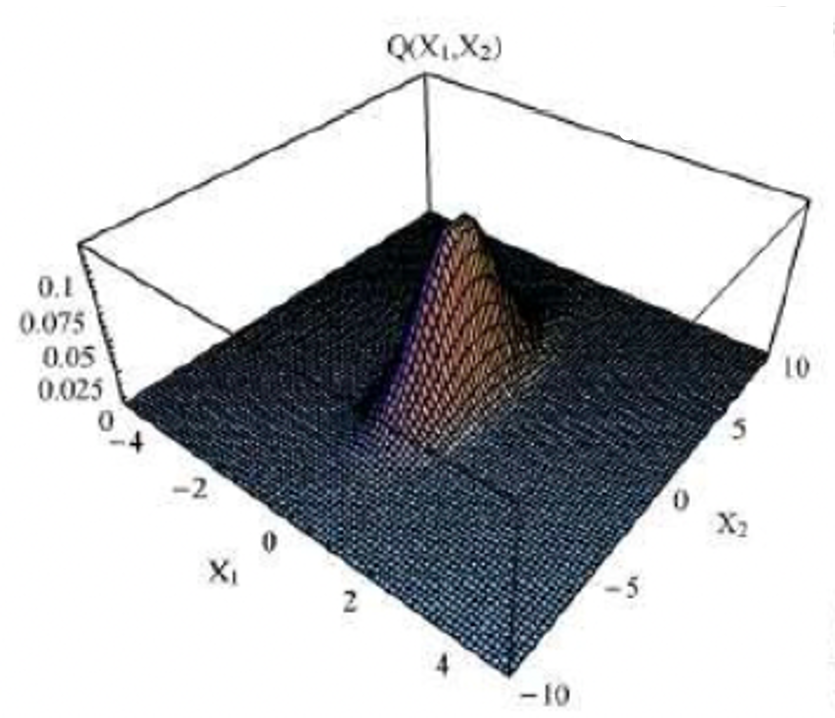
\includegraphics[width=0.95\textwidth]{figs/22.png}
            \end{center}
        \end{column}
      \end{columns}
  \end{frame}

  \begin{frame} 
  \frametitle{}
      例: 已知体系的$Q(\alpha)$函数, 试求$P(\alpha)$函数 \\ 
      \解~ 它们之间存在傳里叶变换关系 
      \[ \begin{aligned}
        Q(\alpha) &= \frac{1}{\pi} \int  d^2 \alpha' P(\alpha') e^{-\left|(\alpha'-\alpha)\right|^2}\\
        &= \frac{1}{\pi} \int  d^2 \alpha' P(\alpha') e^{-\left|\alpha'\right|^2} e^{-\left|\alpha\right|^2} e^{\alpha'\alpha^*  +(\alpha')^* \alpha  } \\ 
        Q(\alpha)e^{\left|\alpha\right|^2} &= \frac{1}{\pi} \int  d^2 \alpha' [P(\alpha') e^{-\left|\alpha'\right|^2}]  e^{\alpha'\alpha^*  +(\alpha')^* \alpha  } \\ 
        P(\alpha') e^{-\left|\alpha'\right|^2} &= \frac{1}{\pi} \int  d^2 \alpha [Q(\alpha)e^{\left|\alpha\right|^2}]  e^{-\alpha'\alpha^*  -(\alpha')^* \alpha  } \\
        P(\alpha')  &= \frac{e^{\left|\alpha'\right|^2}}{\pi} \int  d^2 \alpha [Q(\alpha)e^{\left|\alpha\right|^2}]  e^{-\alpha'\alpha^*  -(\alpha')^* \alpha  } 
      \end{aligned}\] 
  \end{frame}

  \begin{frame} 
    \frametitle{~$Winger$ 表示}
    (1) 对称排序密度算符定义$Winger$函数:
    \[ W(\alpha) =\frac{1}{\pi} \overline{\rho}^{(s)}(\alpha, \alpha^*)\]
    (2) 对称排序算符的均值公式:
    \[ \left\langle F^{(s)} (a, a^{\dagger}) \right\rangle = \int W(\alpha) \overline{F}^{(s)} (\alpha, \alpha^{*}) d^2 \alpha\]
    (3) 相干纯态$\rs{\beta}$的Winger函数:
    \[ W(\alpha) = \frac{2}{\pi} e^{-2\left| (\alpha-\beta) \right|^2}\]
  \end{frame}

  \begin{frame} 
  \frametitle{}
    (4) 纯数态$\rs{n}$的Winger函数:
    \[ W(\alpha) = \frac{2}{\pi} (-1)^n e^{-2\left| \alpha\right|^2} L_n(4\left|\alpha\right|^2)\]
    式中, $L_n$是拉盖尔多项式 \\ {\vspace*{0.3em}}
    (5) 与$P$函数的关系(傅里叶变换)
    \[W(\alpha) = \frac{2}{\pi} \int  d^2 \alpha' P(\alpha') e^{-2\left|(\alpha'-\alpha)\right|^2}\]
  \end{frame}

  \section{3. 特征函数}

  \begin{frame} 
  \frametitle{随机变量的矩}
      设有随机变量$x$, 其对应的可观测量$X$的概率密度为
      \[ \rho (x) \ge 0, \qquad \text{with} ~ \int \rho (x) dx =1\]
      第$n$阶矩定义为:
      \[ \left\langle x^n \right\rangle =  \int x^n \rho (x) dx \]
      如果所有阶的矩$\{\left\langle x^n \right\rangle \}$都知道, 则可求出$\rho (x)$
  \end{frame}

  \begin{frame} 
  \frametitle{特征函数}
     对所有阶的矩加权求和, 可得$e$指数的矩
     \[ \begin{aligned}
      \sum _{n=0} ^ \infty  \frac{(ik)^n}{n!} \left\langle x^n \right\rangle &= \int e^{ikx} \rho (x) dx\\
      &= \left\langle e^{ikx} \right\rangle\\
     \end{aligned}\] 
     由$e$指数的矩定义特征函数
     \[ C(k) \equiv \left\langle e^{ikx} \right\rangle\]
     显然,特征函数与概率密度存在傅里叶变换关系
     \[C (k) = \int e^{ikx} \rho (x) dk \]
     \[\rho (x) = \frac{1}{2 \pi}\int e^{-ikx} C (k) dk \]
  \end{frame}

  \begin{frame} 
  \frametitle{}
     当然,可以从特征函数计算变量的矩
     \[ \left\langle x^n \right\rangle = \left.\frac{1}{i^n} \frac{d^n }{d k^n} C(k)\right|_{k=0} \]
  \end{frame}

  \begin{frame} 
  \frametitle{}
     在量子力学相干表象里,根据算符排序的不同, 可定义三种特征函数
     \[ \begin{aligned}
      C_W (\lambda) & = Tr[\rho e^{\lambda a^{\dagger} -\lambda^* a}] \\ 
      &= Tr[\rho D(\lambda)], \qquad \qquad  \text{(Wigner)} \\
      C_N(\lambda) &= Tr[\rho e^{\lambda a^{\dagger}} e^{ -\lambda^* a}], \qquad  \text{(正规序)}\\
      C_A(\lambda) &= Tr[\rho e^{-\lambda a^{\dagger}} e^{ \lambda^* a}], \qquad  \text{(反正规序)}\\
     \end{aligned}\] 
     三者的关系为:
     \[  C_W (\lambda)  =  C_N(\lambda) e^{- \frac{1}{2}|\lambda|^2} = C_A(\lambda) e^{ \frac{1}{2}|\lambda|^2}\]
     三者的统一定义:
     \[  C(\lambda,s)= Tr[\rho e^{\lambda a^{\dagger} -\lambda^* a + s |\lambda|^2 /2}] \]
     有\[C(\lambda,0) = C_W (\lambda), \quad C(\lambda,1) = C_N (\lambda) , \quad C(\lambda,-1) = C_A (\lambda)\] 
  \end{frame}

  \begin{frame} 
  \frametitle{}
   同理,从特征函数可计算各种排序的算符的矩(均值)
   \[ \begin{aligned}
    \left\langle a^{\dagger m} a ^n \right\rangle = Tr[\rho a^{\dagger m}a ^n ] = \left.\frac{\partial^{(m+n)} }{\partial \lambda ^m  \partial (-\lambda^*)^n } C_N (\lambda) \right|_{\lambda=0}\\
    \left\langle a ^m a^{\dagger n}  \right\rangle = Tr[\rho a ^m a^{\dagger n} ] = \left.\frac{\partial^{(m+n)} }{\partial \lambda ^n  \partial (-\lambda^*)^m } C_A (\lambda) \right|_{\lambda=0}\\
    \left\langle \{a^{\dagger m} a ^n\}_W \right\rangle = Tr[\rho\{a^{\dagger m} a ^n\}_W] = \left.\frac{\partial^{(m+n)} }{\partial \lambda ^m  \partial (-\lambda^*)^n } C_W (\lambda) \right|_{\lambda=0}
   \end{aligned}\] 
  \end{frame}

  \begin{frame} 
  \frametitle{}
   例: 试证明特征函数$C_A (\lambda)$ 与$Q(\alpha)$存在傅里叶变换关系 \\ {\vspace*{0.6em}} 
  \证~ 
  \[ \begin{aligned}
    C_A(\lambda) &= Tr[\rho e^{-\lambda a^{\dagger}} e^{ \lambda^* a}]\\
    &= Tr[e^{ \lambda^* a}\rho e^{-\lambda a^{\dagger}} ]\\
    &= \frac{1}{\pi} \int \left\langle \alpha | e^{ \lambda^* a}\rho e^{-\lambda a^{\dagger}}| \alpha\right\rangle d ^2 \alpha\\ 
    &=  \int Q(\lambda) e^{ \lambda a^{*}-\lambda^* \alpha }  d ^2 \alpha
   \end{aligned}\]
   因此, 
   \[ Q(\alpha) = \frac{1}{\pi^2} \int C_A(\lambda) e^{ \lambda^* \alpha- \lambda a^{*}}  d ^2 \lambda\]
  \end{frame}

  \begin{frame} 
  \frametitle{}
     同理,
     \[ P(\alpha) = \frac{1}{\pi^2} \int C_N(\lambda) e^{ \lambda^* \alpha- \lambda a^{*}}  d ^2 \lambda\]
     \[ W(\alpha) = \frac{1}{\pi^2} \int C_W(\lambda) e^{ \lambda^* \alpha- \lambda a^{*}}  d ^2 \lambda\]
     代入
     \[  C_W (\lambda)  =  C_N(\lambda) e^{- \frac{1}{2}|\lambda|^2}\]
     有 \[ W(\alpha) = \frac{1}{\pi^2} \int C_N(\lambda) e^{- \frac{1}{2}|\lambda|^2} \exp(\lambda^* \alpha- \lambda a^{*})  d ^2 \lambda\]

    因此,从特征函数,可以直接得到各概率函数 $ W(\alpha), P(\alpha), Q(\alpha)$表示
  \end{frame}

  \begin{frame} 
  \frametitle{}
       \begin{center}
         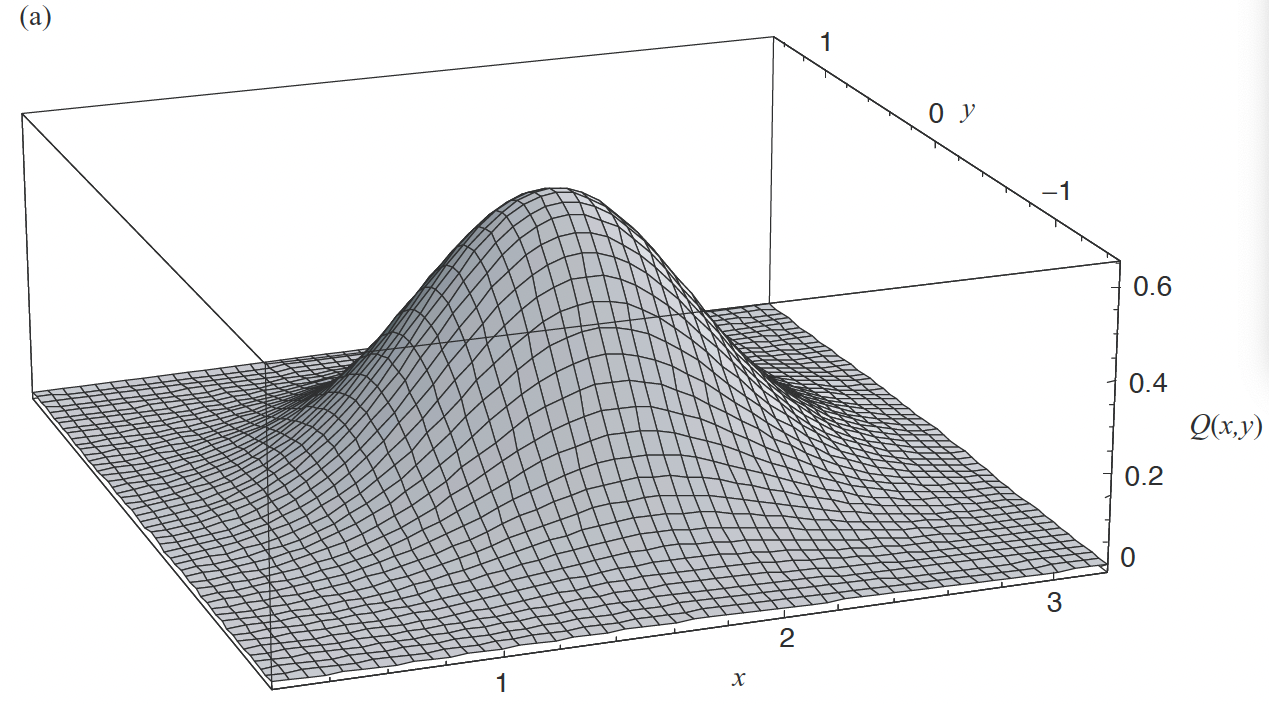
\includegraphics[width=0.8\textwidth]{figs/2022-06-16-12-43-48.png}
       \end{center}
       一个平均光子数为10的相干态的$Q(\alpha)$函数 ($\alpha=x+iy$)
  \end{frame}

  \begin{frame} 
    \frametitle{}
         \begin{center}
           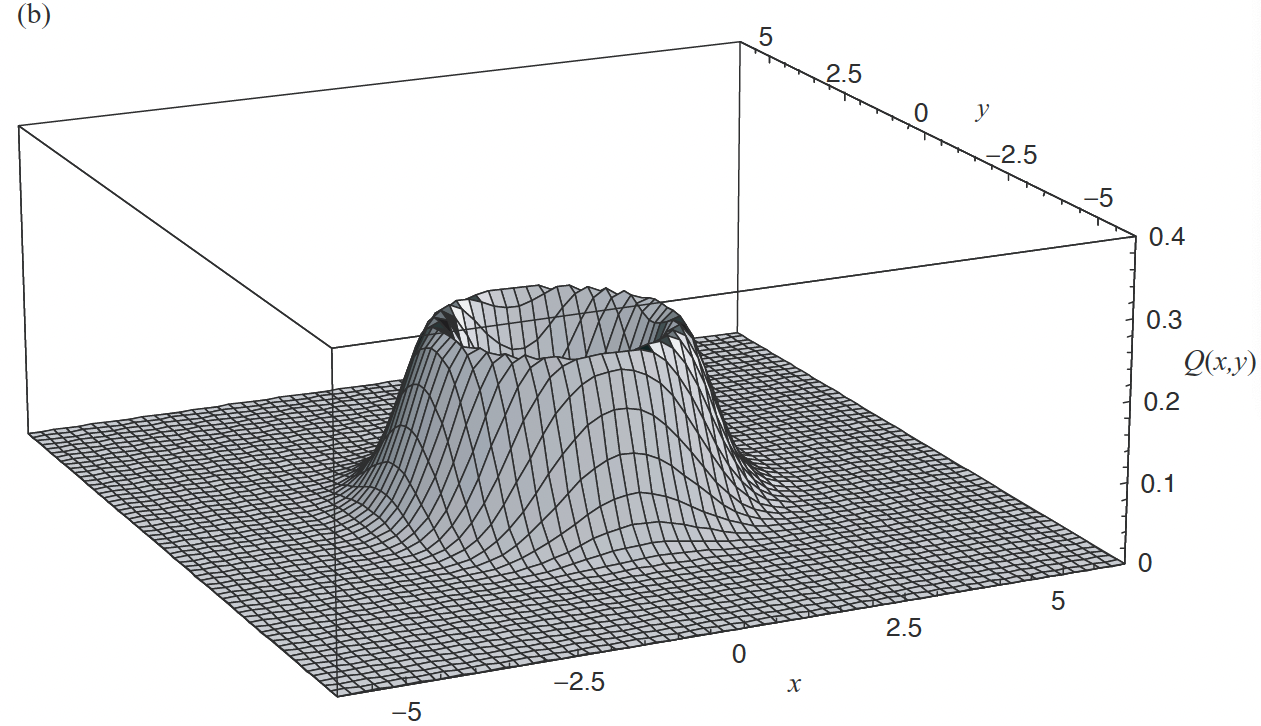
\includegraphics[width=0.8\textwidth]{figs/2022-06-16-12-48-42.png}
         \end{center}
         数态$\rs{n}=\rs{3}$的$Q(\alpha)$函数 ($\alpha=x+iy$)
    \end{frame}

    \begin{frame} 
      \frametitle{}
           \begin{center}
             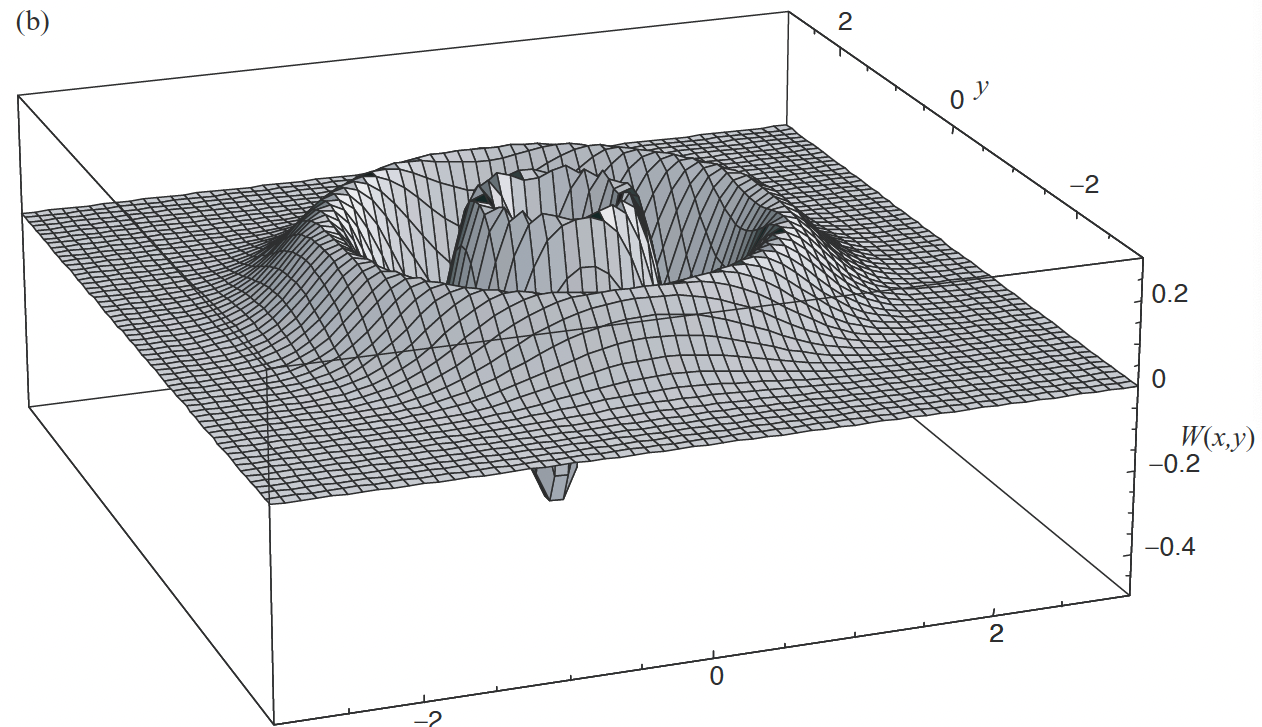
\includegraphics[width=0.8\textwidth]{figs/2022-06-16-12-50-28.png}
           \end{center}
           数态$\rs{n}=\rs{3}$的W函数. 存在振荡和“负概率”区域(非经典效应)
      \end{frame}
   %%%%%%%%%%%%%%%%%%%%%%%%%%%%%%%%%%%%%%%%%%%%%%%%%%%%%%%%%%%%%%%%%%%
   \begin{frame} 
       \frametitle{课外作业}
       \begin{enumerate}
           \item 试证明  \[Tr f(a, a^{\dagger}) = \frac{1}{\pi}Tr \int f(a, a^{\dagger}) \rl{\alpha}{\alpha} d^2 \alpha\]
           \item 试证明  \[Tr f(a, a^{\dagger}) = \frac{1}{\pi}Tr \int \ls{\alpha} f(a, a^{\dagger}) \rs{\alpha} d^2 \alpha\]
           \item 设压缩态为$\rs{\beta,\xi}$, 求光子数分布:
           \[ P(n) = \left| \lr{n}{\beta,\xi} \right|^2\]
       \end{enumerate}
   \end{frame}
   %%%%%%%%%%%%%%%%%%%%%%%%%%%%%%%%%%%%%%%%%%%%%%%%%%%%%%%%%%%%%%%%%%%